\rightline{{\rm \textit{Ch-ch-ch-ch-changes}}}
\rightline{{\rm \textit{Turn and face the strange}}}
\rightline{{\rm \textit{Ch-ch-changes}}}
\rightline{{\rm \textit{There's gonna have to be a different man}}}

\rightline{{\rm --- David Bowie}}

\section{Derivatives model change}

In studying fluid motion, we are inherently interested in change in various quantities associated with the fluid. For example, simply because of fluid moving around, its local density or its local temperature might change. In that sense, the main goal of the science of fluid dynamics is to describe that change. We would like to know how flow affects various fluid properties such as density, $\rho$, pressure, $p$, temperature, $T$, or even fluid composition for multicomponent mixtures.

Changes are mathematically modeled by derivatives. Derivative explains how much one variable, say $\phi_1$, changes when we change some other variable, say $\phi_2$, and we express this in mathematical terms as
\begin{equation*}\label{eq:change-d}
\frac{d \phi_1}{d \phi_2} \, ,
\end{equation*}
where the letter $d$ stands for \textit{the change of...} and is later followed by the variable that we are speaking of. So really the above ratio means that there is \textit{this much} change in variable $\phi_1$ per \textit{this much} change in variable $\phi_2$. You can also think of this ratio as \textit{this much} change in variable $\phi_1$ per \textit{unit} change in variable $\phi_2$.

In fluid dynamics, you will find that we are most interested in two types of changes: \textit{change in time} and \textit{change in space} (position). Since we live in the three-dimensional space with a time arrow, it is justifiable why these two have the biggest popularity, right? Therefore, you will most often encounter $dt$ or $dx$, $dy$, $dz$ in the denominator of various forms of Eq.~(\ref{eq:change-d}).

Let's take pressure, $p$, as an example. When we write
\begin{equation*}\label{eq:change-p}
\frac{d p}{d t} \, ,
\end{equation*}
you can read this as: there is this much change in $p$ per this much change in $t$.
Similarly, you may encounter expressions like
\begin{equation*}\label{eq:change-p}
\frac{d p}{d t} \, ,
\end{equation*}


There is also another mathematical expression for a derivative and it is:
\begin{equation*}\label{eq:change-partial}
\frac{\partial \phi_1}{\partial \phi_2} \, .
\end{equation*}
The operator $\partial$ (called ''partial`` or ''del``) also stands for \textit{the change of...} but it also gives you a hint that the variable $\phi_1$ can change with the change of variables other than $\phi_2$. Perhaps it can also change with some $\phi_3$ and $\phi_4$, even though in this particular ratio from Eq. (\ref{eq:change-partial}) we are only interested in the change with respect to $\phi_2$.

\section{What does it mean for a quantity to change in time and in space?}


\subsection{Steady-state case and a time derivative}

\section{Convention for the sign of a derivative}

For the purpose of this demonstration we will look at the derivative $\frac{dp}{dx}$ -- change in pressure per change in the $x$-axis position -- which is often encountered in fluid dynamics. We will lay the ground for what does it mean for this derivative to be positive, negative or zero, and why the reasoning makes sense.

Suppose that the initial point is marked with \textcolor{myblue}{$(i)$} and it is always a point at coordinate $x$. The point to which we move after one space-step, the final point, is marked with \textcolor{myblue}{$(f)$} and is either at $x+dx$ or $x - dx$ coordinate, depending on the positive or negative change that we decide to make. The direction of the change on the $x$-axis is marked with a blue arrow.

\begin{figure}[H]
\begin{subfigure}[t]{.46\textwidth}
\centering
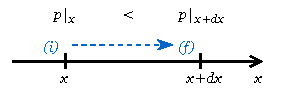
\includegraphics[scale=1]{dp-dx-pos-neg.pdf}
\caption{$\frac{dp}{dx} > 0$ with positive change in $x$.}
\end{subfigure}
\begin{minipage}[t]{.07\textwidth}
$ $
\vspace*{1.5cm}
\end{minipage}
\begin{subfigure}[t]{.46\textwidth}
\centering
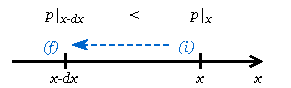
\includegraphics[scale=1]{dp-dx-neg-neg.pdf}
\caption{$\frac{dp}{dx} > 0$ with negative change in $x$.}
\end{subfigure}
\begin{subfigure}[t]{.46\textwidth}
\centering
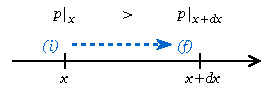
\includegraphics[scale=1]{dp-dx-pos-pos.pdf}
\caption{$\frac{dp}{dx} < 0$ with positive change in $x$.}
\end{subfigure}
\begin{minipage}[t]{.08\textwidth}
$ $
\end{minipage}
\begin{subfigure}[t]{.46\textwidth}
\centering
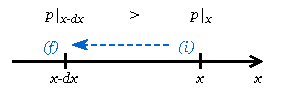
\includegraphics[scale=1]{dp-dx-neg-pos.pdf}
\caption{$\frac{dp}{dx} < 0$ with negative change in $x$.}
\end{subfigure}
\caption{Sign of the $\frac{dp}{dx}$ derivative versus directions of change along the $x$-axis.}
\label{fig:dp-dx-signs}
\end{figure}

We will now find out for all cases which pressure, at \textcolor{myblue}{$(i)$} or at \textcolor{myblue}{$(f)$} must be larger. Our aim is to show that situations (a) and (b) in Figure \ref{fig:dp-dx-signs} must be equivalent -- they explain the same physical phenomena. In both of these cases we will show that the pressure is increasing with the increasing $x$-coordinate, independent of whether we decide to take a step to the right or to the left of our initial point \textcolor{myblue}{$(i)$}. 

We will show the analogical result can be said about situations (c) and (d) but in this case the pressure is decreasing with the increasing $x$-coordinate.



\subsection{Closing note}

The analysis done in this section is often necessary in order to find out whether or not to ''put a minus sign`` in front of expressions. For instance, as we will show later in the text, such reasoning can help us understand why there is a minus sign in the Euler equation for a fluid element experiencing pressure force: $dp = - \rho \upsilon d \upsilon$. Oftentimes, the sign of a derivative tells an important information about the nature of the physical phenomena.





